%! TEX root = 0-main.texj
\chapter{Rigid Body Dynamics}
\section{Inertia Tensor}
Consider the rotation of a rigid body about a point \(O\neq \vb r_{cm}\), which is separated from the origin in a fixed frame by \(\vb R\). The position of a mass element can be written as \(\vb r_\alpha\). Because it is a rigid body, in the frame of the rigid body, we have \(\at{\der{\vb r_\alpha}{t}}{rot}=0\). The velocity of the mass element in the fixed frame, 
\[\vb v_\alpha ' = \dot{\vb R} + \vv\omega\times\vb r_\alpha\]
The angular momentum about the fixed origin, \(O'\) can be given
\begin{align*}
	\vb L'_T &= \sum_\alpha m_\alpha(\vb R+\vb r_\alpha)\times\vb v_\alpha'\\
		 &=\sum_\alpha m_\alpha \vb R \times \vb V+\left(\sum_\alpha m_\alpha \vb r_\alpha\right)\times V + \vb R\times \left(\vv\omega\times \sum_\alpha m_\alpha \vb r_\alpha\right) + \sum_\alpha m_\alpha\vb r_\alpha\times(\vv \omega\times\vb r_\alpha)\\
		 &=M(\vb R+\vb r_{cm})\times \vb V + M\vb R\times \vb v_{cm}+\sum_\alpha m_\alpha \vb r_\alpha \times (\vv \omega \times \vb r_\alpha)
\end{align*}
The first term is the angular momentum due to the object veloctiy wrt the centre of mass, the second term the angular momentum of due to the motion of the centre of mass, while the last term is the angular momentum wrt the origin \(O\). Thus, we define
\[\vb L_{body} \equiv \vb L = \sum_\alpha m_\alpha \vb r_\alpha \times (\vb \omega\times\vb r_\alpha)\]
Using BAC-CAB, can rewrite this as
\begin{equation}
	\vb L = \sum_\alpha m_\alpha r_\alpha^2 \vb \omega - \sum_\alpha m_\alpha (\vb r_\alpha*\vv\omega)\vb r_\alpha
\end{equation}
Let \(\vb r_\alpha = x_{i}^{(\alpha)}\e{i}\) and \(\vv\omega = \omega_i e_i\). Then,\footnote{In class, we use the notation \(x_{\alpha i} = x^{(\alpha)}_i\)}
\[L_j = \sum_\alpha m_\alpha \left[\left(\sum_{k=1}^3x^{(\alpha)}_kx^{(\alpha)}_k\right)\omega_j - \left(\sum_i x^{(\alpha)}_i\omega_i\right) x^{(\alpha)}_{j}\right]\]
We see from the second term that \(\vb L\) is not always parallel to \(\vv\omega\). Let \(\omega_j = \sum_i \delta_{ij}\omega_i\). Then, we can rewrite \(L_j\) as
\begin{align*}
	L_j &= \sum_\alpha m_\alpha\sum_i\left[\left(\sum_k x^{(\alpha)}_kx^{(\alpha)}_k\delta_{ij}\right)-x^{(\alpha)}_ix^{(\alpha)}_j\right]\omega_j\\
	    &=\sum_i \omega_i \sum_\alpha m_\alpha \left[\left(\sum_k x^{(\alpha)}_kx^{(\alpha)}_k\delta_{ij}\right)-x^{(\alpha)}_ix^{(\alpha)}_j\right]
\end{align*}
We thus define the \emph{inertia tensor}\footnote{Note, that this is not the \emph{moment of inertia tensor}.}
\begin{equation}
	I_{ij}=\sum_\alpha m_\alpha \left[\left(\sum_k x_k^{(\alpha)}x_k^{(\alpha)}\right)\delta_{ij}-x_{i}^{(\alpha)}x_j^{(\alpha)}\right]
\end{equation}
such that
\[\vb L = \stackrel{\leftrightarrow}{\vb I} \vv\omega\]
or
\[L_i = \sum_jI_{ij}\omega_j\]
It is easy to see that \(I_{ij} =I_{ji}\), so the tensor is \emph{symmetric}. Thus, there are only 6 independent components to the tensor, rather than \(3\times 3=9\).

The diagonal elements are known as the moments of inertia, where \(I_{ii}\) gives the moment about the \(x_i\) axis, while the off-diagonal elements are the products of inertia. 

We can extend our definition of the inertia tensor to allow \emph{continuous} rigid bodies in the natural way:
\begin{equation}
	I_{ij} = \int_V\d{m} \left[x^2\delta_{ij} - x_ix_j\right] = \int_V\rho\d[3]{x}\left[x^2\delta_{ij}-x_ix_j\right]
\end{equation}

\subsubsection{Spinning Dumbell}
Consider a spinning dumbell, which consists of two point masses \(m\) connected by a massless rod length \(2a\)and spinning about an axis through the centre of mass, but is not necessarily at a angle aligned to the rod.
\begin{center}
	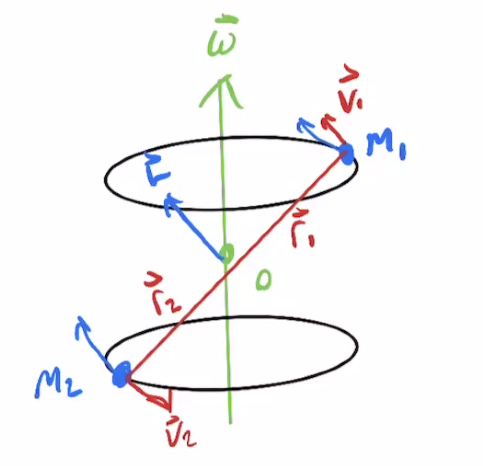
\includegraphics[scale = 0.5]{lwcounter.png}
\end{center}

Let \(\vv\omega = \omega\hat z\), and the rod at angle \(\theta\) to \(\hat z\). Then, we can write \(\vb a_1 = a(\sin\theta\hat y + \cos\theta\hat z)\) and \(\vb a_2 = -a(\sin\theta\hat y + \cos\theta\hat z)\) where at a time \(t=0\), we fix \(x\) such that \(a_x=0\). Then, the angular momentum of the system is given
\[\vb L = 2m\omega a^2\sin\theta(\sin\theta\hat z- \cos\theta \hat y)\]
Note, that \(\vb L\parallel \vv \omega\) iff \(\cos\theta = 0\then\theta = \frac{\pi}{2}\).

As we allow the dumbell to evolve in time, we need to consider the inertia tensor. For consistency, let \(\phi\) be the angle from the \(y\) axis, rather than from the \(x\) axis, as would be expected from normal spherical coordinates. We then have
\[-\vb a_2 = \vb a_1 = a\vect{\sin\theta\sin\phi, \sin\theta\cos\phi,\cos\theta}\]
as the positions of the two masses. Our inertia tensor then becomes
\[I = 2ma^2\begin{bmatrix}
	\sin^2\theta\cos^2\phi+\cos^2\theta & -\sin^2\theta\sin\phi\cos\phi & -\sin\theta\cos\theta\sin\phi\\
			-\sin^2\theta\sin\phi\cos\phi & \sin^2\theta\sin^2\phi+\cos^2\theta & -\sin\theta\cos\theta\cos\phi\\
			-\sin\theta\cos\theta\sin\phi & -\sin\theta\cos\theta\cos\phi & \sin^2\theta
\end{bmatrix}\]
If \(\dot\phi=0\), then we are in the body system, using \emph{body coordinates}. Thus, the problem reduces to what we had previously considered. As before, fix \(\phi=0\), so
\[I = 2ma^2 \begin{bmatrix}
	1 & 0 & 0\\
	0 & \cos^2\theta & -\sin\theta\cos\theta \\
	0 & -\sin\theta\cos\theta & \sin^2\theta
\end{bmatrix}\]
Thus, we see that
\[\vb L = \stackrel{\leftrightarrow}{\vb I}\vv\omega = 2ma^2\omega \sin\theta\left(\sin\theta\hat z-\cos\theta\hat y \right)\]
which matches our previous result.

If we, however, take \(\dot\phi\neq0\), such as in the fixed frame, the angular momentum instead rotates around the \(z\) axis. This rotation is called \emph{precesion}. Because we see that the angular momentum is changing, there must be a torque being applied to maintain the precession. Using the relation between the time derivative of vectors in moving frames and fixed frames, we obtain that the torque becomes
\[\vv\tau = \underbrace{\at{\der{\vb L}{t}}{\text{fixed}}}_{=0}+\vv\omega\times \vb L\]
\[\vv\tau = 2\omega^2ma^2\sin\theta\cos\theta\hat x\]
Trivially, we see there is no torque when \(\theta = 0, \pi/2\).

\subsection{Principle Axes of Inertia}
Note, that because the inertia tensor has a symmetric matrix representation, that there exists an orthonormal basis such that the inertia tensor is diagonal; these axes are known as the \emph{principle axes}. We then write, along the principle axes, that
\[L= I_{i}\omega_i\]
Finding these principle axes is a standard eigenvalue problem.
\[\det(\stackrel{\leftrightarrow}{\vb I}-I_i\mathbbm1)=0\]
The eigenvalues \(I_i\) are the \emph{principle moments}, and the eigenvectors are the \emph{principle axes}.

\subsection{Kinetic Energy}
Recall that the kinetic energy is defined
\[T = \frac{1}{2}\sum_{\alpha}m_\alpha v_\alpha^2\]
Substituting \(v_\alpha = \omega\times r_\alpha\), we obtain
\begin{align*}
	T_{\text{rot}} &= \frac{1}{2}\sum_\alpha m_\alpha (\omega\times r_\alpha)\times (\omega\times r_\alpha)\\
		       &=\frac{1}{2}m_\alpha\omega*(r_\alpha\times(\omega\times r_\alpha))\\
		       &=\frac{1}{2}\omega*\sum_\alpha m_\alpha (r_\alpha\times (\omega\times r_\alpha))
\end{align*}
Recognizing the final sum, we see that 
\begin{equation}
	T_{\text{rot}} = \frac{1}{2} \vv\omega \times \vb L = \frac{1}{2}\vv\omega * \stackrel{\leftrightarrow}{\vb I}\vv\omega
\end{equation}
Expanding the second representation, we obtain
\begin{equation}
	T_{\text{rot}} = \frac{1}{2}\sum_{ij} \omega_iI_{ij}\omega_j
\end{equation}

\subsection{Steiner's Parallel Axis Theorem}
Consider a stationary coordinate system at a distance \(\vb a\) away from the CoM coordinate system and with parallel. Trivially, if \(X\) is the second coordinate system, and \(x\) is the first coordiate system, we can write \(X=x+a\). When we plug this into the formula for the inertia tensor in \(X\), we can simplify to obtain
\begin{equation}
	J_{ij} = I_{ij} + M(a^2\delta_{ij}-a_ia_j)
\end{equation}
where \(I_{ij}\) is the CoM inertia tensor, and the second term is the inertia tensor of a point mass M in the displaced coordinate system.

\subsection{Changing Axes}
Let \(x' = \Lambda x\). Then, we can transform the inertia tensor via
\[I' = \Lambda I \Lambda^{-1}\]
What systems satisfy \(I' = I\)? We see trivially that with principle axes \(x,y,z\), we can write
\[I = \left(\sum_{\alpha}m_\alpha r_\alpha^2\right)\mathbbm 1 - \left(\sum_\alpha m_\alpha r\tp r\right)\]
Or,
\[I =I_0 \mathbbm 1 - \sum_\alpha m_\alpha r^{\tp 2}\]
Define an arbitrary scaling transformation \(x,y,z\to a_xx, a_yy, a_zz\). Then,
\[I_{ii}' = I_0' - a_i^2\sum_\alpha m_\alpha r_{\alpha,i}^2\]
Where \(I_0\) doesn't necessarily equal \(I_0'\). Choosing \(a,b,c\) such that \(I' = I'\mathbbm 1\), we see that \emph{any body} can be ``squashed'' until they have a spherical inertia tensor.

\section{Euler Angles}
Similar to how a plane has pitch, roll, and yaw, a set of three \emph{Eulerian Angles} which completely define the orientation of the object. These angles, \(\f,\theta,\p\), along with the Euler-Lagrange equations will allow us to find the equations of motion of a ``tumbling'' object.

\subsubsection{Force-Free}
Consider the case wherer there is no translational kinetic energy. We will define our system by composing three rotations\footnote{In lecture, the \(x'''\) and \(x'\) labels are flipped. I chose to start with \(x'''\) rather than \(x'\) for a nice progression of each transformation ``deleting'' a prime.} First, we will rotate by \(\f\) about the \(x_3'''\) axis. We then obtain our first transformation as
\[ \begin{bmatrix}
	x_1''\\x_2''\\x_3''
\end{bmatrix}= \begin{bmatrix}
\cos\phi & \sin\phi & 0\\
-\sin\phi & \cos\phi & 0 \\
0&0&1
\end{bmatrix} \begin{bmatrix}
	x_1'''\\x_2'''\\x_3'''
\end{bmatrix}\]

We make our next rotation by \(\theta\) about \(x_1''\). This gives
\[ \begin{bmatrix}
	x_1'\\ x_2'\\x_3'
\end{bmatrix}=
\begin{bmatrix}
	1 & 0 & 0\\
	0 & \cos\theta & \sin\theta\\
	0 & -\sin\theta & \cos\theta
\end{bmatrix}
\begin{bmatrix}
	x_1''\\x_2''\\x_3''
\end{bmatrix} \]

Finally, we rotate by \(\p\) about \(x_3'\), so
\[ \begin{bmatrix}
	x_1\\x_2\\x_3
\end{bmatrix}= \begin{bmatrix}
\cos\p & \sin\p & 0\\
-\sin\p & \cos\p & 0 \\
0&0&1
\end{bmatrix} \begin{bmatrix}
	x_1'\\x_2'\\x_3'
\end{bmatrix}\]
Note that the three vectors \(\dot\f,\dot\theta,\dot\p\) are \emph{not} orthogonal. However, there is an interesting line called the \emph{line of nodes} which points along the \(\dot\theta\) direction, and is the intersection between the \(x_1x_2\) and \(x_1'''x_2'''\) planes.
When we compound these three rotations, we obtain the transformation matrix from \(x'''\to x\) as
\begin{equation}
	\begin{bmatrix}
		\cos\p\cos\f-\cos\theta\sin\f\sin\p & \cos\p\sin\f + \cos\theta\cos\f\sin\p & \sin\p\sin\f\\
		-\sin\p\cos\f - \cos\theta\sin\f\cos\p & -\sin\p\sin\f + \cos\theta\cos\f\cos\p& \cos\p\sin\theta\\
		\sin\theta\sin\f & -\sin\theta\cos\f & \cos\theta
	\end{bmatrix}
\end{equation}

\subsection{Euler's Equations of Motion}
To use the Euler-Lagrange equations, we must know how the coordinates change with time. Trivially, we have 
\begin{equation}
	\dot\p = \dot\p x_3
\end{equation}
The second velocity \(\dot\theta\) lies along the line of nodes; it is the intersection of the \(x_1x_2\) and \(x_1'''x_2'''\) axes. It is \emph{in} the \(x_1x_2\) plane, but is offset at an angle \(\p\) down from \(x_1\). Thus,
\begin{equation}
	\dot\theta = \dot\theta \cos\phi \hat x_1 -\dot \theta \sin\theta \hat x_2
\end{equation}
Some work needs to be done for our final angle, however. After compounding the two rotations \(R_\p\circ R_\theta\), we obtain
\begin{equation}
	\dot\f = \dot \phi \sin\theta\sin\p \hat x + \dot\phi \sin\theta\cos\p + \dot\phi\cos\theta
\end{equation}
Note that our first angle is akin to a 1D spherical (linear) coordinates, the second akin to 2D spherical (polar) coordinates with angle \(\theta\), and the third akin to 3D spherical coordinates, with polar angle \(\theta\) and azimuthal angle \(\p\).

Our overall angular velocity is given
\begin{equation}
	\omega = \dot\p + \dot\theta +\dot\f
\end{equation}

To go from Lagrange's equations of motions to Euler's equations, we use our three angles as generalized coordinates. First, we set our reference frame with respect to the principle axes, so our inertia tensor is diagonal. Further, considering force-free motion, we can fix \(U=0\). We can consequently write our Lagrangian as
\[L = T = \frac{1}{2}\sum_i I_i\omega_i^2\]
Beginning with \(\p\), 
\begin{align*}
	0 &= \pder{L}{\p}-\der{}{t}\pder{L}{\dot\p}\\
	  &= \pder{T}{\p}-\der{}{t}\pder{T}{\dot\p}\\
	  &= \sum_{i}\pder{T}{\omega_i}\pder{\omega_i}{\p}-\der{}{t}\pder{T}{\omega_i}\pder{\omega_i}{\dot\p}\\
	  &= \left(\sum_i L_i *\pder{\omega_i}{\p} \right) - \der{}{t} L_3
\end{align*}

Plugging in our values for \(\omega\), we obtain the Euler Equations of Motion
\begin{subequations}
	\begin{align*}
		(I_2-I_3)\omega_2\omega_3-I_1\dot\omega_1&=0\\
		(I_3-I_1)\omega_3\omega_1-I_2\dot\omega_2&=0\\
		(I_1-I_2)\omega_1\omega_2-I_3\dot\omega_3&=0
	\end{align*}
\end{subequations}
However, when we have torque, we have
\[N = \at{\der{L}{t}}{\text{fixed}} = \at{\der{L}{t}}{\text{body}}+\omega\times L\]
Because we chose \(I\) to be diagonal, we know
\[L_i = I_i\omega_i\then \dot L_i = I_i\dot\omega_i\]
we can then rewrite our Euler equations of motion as
\begin{subequations}
	\begin{align}
		I_1\dot\omega_1-(I_2-I_3)\omega_2\omega_3&=\tau_1\\
		I_2\dot\omega_2-(I_3-I_1)\omega_3\omega_1&=\tau_2\\
		I_3\dot\omega_3-(I_2-I_1)\omega_1\omega_2&=\tau_3
	\end{align}
\end{subequations}
or, in general,
\begin{equation}
	(I_i-I_j)\omega_i\omega_j - \sum_k (I_k\dot\omega_k-N_k)\varepsilon_{ijk}=0
\end{equation}
\section{Symmetric Top}
Consider a top with
\[I_1=I_2 \neq I_3\]
In the absense of force, we can set \(\tau = 0\). Plugging into the Euler EoM,
\begin{align*}
	0&=I_3\dot\omega_3\\
	0&=(I_1-I_3)\omega_2\omega_3-I_1\dot\omega_1\\
	0&=(I_3-I_1)\omega_1\omega_3-I_1\dot\omega_2
\end{align*}
Simplifying, we obtain
\[\dot\omega_1 = -\frac{I_3-I_1}{I_1}\omega_3\omega_2\equiv -\Omega\omega_2\]
\[\dot\omega_2 = +\frac{I_3-I_1}{I_1}\omega_3\omega_1\equiv +\Omega\omega_1\]
where \(\Omega = \frac{I_3-I_1}{I_1}\omega_3\). A prolate object (such as a can of red bull) will have \(\Omega<0\), while an oblate object (such as a frisbee) will have \(\Omega>0\). Let
\(q = \omega_1+i\omega_2\). Then, our differential equation becomes
\[\dot q -i\Omega q =0\]
or 
\[q = Ae^{i\Omega t}\]
with 
\[\omega_1 = A\cos\Omega t\]
\[\omega_2 = A\sin\Omega t\]
Thus, we see that \(\vv\omega\) precesses about \(x_3\) with angular velocity \(\Omega\).

Further, because there is no torque or force, the kinetic energy is constant, so the angle \(\beta\) between \(\vb L\) and \(\vv\omega\) is constant. Further, we can show that 
\[\vb L*(\vv\omega\times\e3) = 0\]
so these three vectors are all coplanar.

\diagram{}

We can imagine this scenario as two cones rolling about each other. The axis of one cone is the fixed \(x'_3\) direction, or the \(\vb L\) direction, while the other is the body \(x_3\) direction. Of course, the angle between these two axes is the Eulerian angle \(\theta\). Finally, the point of contact of these cones is along the angular velocity vector, \(\vv\omega\). We can find the angle \(\alpha\) between the angular velocity \(\vv\omega\) and the body axis \(x_3\) by using the relation \(L = I\omega\) in body coordinates. Thus, we obtain the equations
\[L\sin\theta = I_1\omega \sin\alpha\]
\[L\cos\theta = I_3\omega\cos\alpha\]
so we obtain
\[\tan\theta = \frac{I_1}{I_3}\tan\alpha\]
Recall that if \(I_1 = I_2>I_3\) our object is prolate and \(\theta>\alpha\). If \(I_1=I_2< I_3\), our object is oblate and \(\theta<\alpha\). We rotate the body cone along \(x'_3\) to obtain the precession; we see that if \(\alpha>\theta\) then this is akin to rolling an object inside of another object, and the precession is in the opposite direction---this is consistent with the angular velocity of the precession \(\Omega\) having negative sign for an oblate object.

\diagram{}

Now we wish to consider the precession of \(x_3\) about \(\vb L\) (this is in contrast to what we calculated earlier, the precession of \(\vv \omega\) about \(x_3'\)). The precession turns out to have angular velocity \(\dot\phi\), as this is the angular velocity about the \(x_3'\) axis.

Fixing \(\psi=0\), we see that when we plug into the expansion of \(\omega\), we have
\[\omega_2 = \dot\phi\sin\theta\]
so
\[\dot\phi = \frac{\omega_2}{\sin\theta} = \frac{\omega\sin\alpha}{\sin\theta} = \frac{\omega \frac{L_2}{I_1\omega}}{\frac{L_2}{L}} = \frac{L}{I_1}\]
where we substituted \(\sin\alpha = L_2/I_1\omega\) and \(\sin\theta = L_2/L\) from earlier.

\subsection{Fixed Point}
Consider a top of mass \(M\) at an angle \(\theta\) with its tip fixed at the origin in a gravitational field. The centre of mass is located at a vector \(\vb h\) from the origin. The top rotates at a rate \(\dot\psi\hat x_3\) and precesses with \(\dot\phi \hat x_3'\).

By substituting what we know about the components of \(\omega\), we can compute the kinetic energy as
\[T = \frac{1}{2}I_1(\dot\phi^2\sin\theta+\dot\theta^2)+\frac{1}{2}I_3(\dot\phi\cos\theta+\dot\psi)^2\]
Trivially, the potential energy is
\[U = Mgh\cos\theta\]
so
\[L = \frac{1}{2}I_1(\dot\phi^2\sin\theta+\dot\theta^2)+\frac{1}{2}I_3(\dot\phi\cos\theta+\dot\psi)^2- Mgh\cos\theta\]
From Euler-Lagrange,  we see that if \(\pder{L}{x} = 0\) then \(\der{}{t}\pder{L}{\dot x}=0\) and so that coodinate is a constant of the motion. Trivially, we see that this is the case for both \(\phi\) and \(\psi\), so \(p_\f\) and \(p_\p\) are conserved momenta. This corresponds to no torque along \(x_3\) or \(x_3'\). These angular momenta can be written explicitly as
\[p_\f = \pder{L}{\dot\phi} = (I_1\sin^2\theta+I_3\cos^2\theta)\dot\phi + I_3\dot\psi\cos\theta\]
\[p_\p = I_3(\dot\p+\dot\f\cos\theta)\]
Solving for \(\dot\p\),
\[\dot\p = \frac{p_\p - I_3\dot\f \cos\theta}{I_3}\]
Using this expression we can then find \(\dot\f\),
\[\dot\f = \frac{p_\f-p_\p\cos\theta}{I_1\sin^2\theta}\]
and reinsert to into \(\dot\p\) to get
\[\dot\p = \frac{p_\p}{I_3}-\frac{(p_\f-p_\p\cos\theta)\cos\theta}{I_1\sin^2\theta}\]

However, we see that both \(\dot\p\) and \(\dot\f\) are not constant, as they are functions of \(\theta(t)\); the variation in \(\theta\) is known as \emph{nutation}, In principle, we can solve for \(\theta\) directly, but it is easier to consider an effective potential instead. In the toal energy,
\[E = \frac{1}{2}\omega * I\omega +U\]
we see that the term \(\frac{1}{2}I_3\omega^2_3 = \frac{p_\p^2}{2I_3}\) is a constant of the motion, \(E\) is conserved, and thus we can define \(E' = E-\frac{1}{2}I_3\omega_3^2\) as a conserved quantity. Substituting in our expression of \(\dot\phi\) into \(\omega_1^2+\omega_2^2=\dot\phi^2\sin^2\theta+\dot\theta^2\) to obtain
\[E' = \frac{1}{2}I_1\dot\theta^2 + \frac{(p_\f - p_\p\cos\theta)^2}{2I_1\sin^2\theta}+Mgh\cos\theta\]
so we obtain the effective potential that governs \(\theta\) as
\[V(\theta) = \frac{(p_\f - p_\p\cos\theta)^2}{2I_1\sin^2\theta}+Mgh\cos\theta\]
Of course, we can use the equation
\[t(\theta) = \int\frac{\d\theta}{2/I_1[E'-V(\theta)]}\]
and \(\theta(t)\) can be obtained by inverting.

If we have \(E'=V_{\min}\), then we see that \(\theta(t)=\dot\theta\), and the precession \(\dot\phi\) is a constant. Minimising \(V(\theta)\), we find that
\[0 = \pder{V}{\theta} = \frac{-\cos\theta_0 (p_\f-p_\p \cos\theta_0)^2+p_\p(p_\f-p_\p\cos\theta_0)\sin^2\theta_0}{I_1\sin^3\theta_0}-Mgh\sin\theta_0\]
Substituting 
\[\beta = \dot\f I_1\sin^2\theta = p_\f-p_\p\cos\theta_0\]
we can simplify as a quadratic in \(\beta\):
\[0 = (-\cos\theta_0)\beta^2 + p_\p \sin^2\theta_0 \beta - MghI_1\sin^4\theta_0\]
so we can use the quadratic formula to find \(\beta\). In particular, the top is only stable if \(\beta\) is real; thus our stability condition is given by the discriminant.
\[\beta = \frac{p_\p\sin^2\theta_0}{2\cos\theta_0}\left(1\pm \sqrt{1-\frac{4 MghI_1\cos\theta_0}{p_\p^2}}\right)\]
thus, our stability condition is given
\[p_\p^2\geq 4MghI_2\cos\theta_0\]
This is always satisfied when \(\theta_0\geq\pi/2\). Note that this corresponds to the top dangling from the ceiling. If this is true, then the top will always precess; there is no minimum condition for \(p_\p\).

Considering the more restricive case that \(\theta_0\le\pi/2\) we can substitute our value for \(p_\p  =I_3(\dot\p+\dot\f\cos\theta) = I_3\omega_3\). Thus, we see that this stability condition translates to
\[\omega_3\geq \frac{\sqrt{4MghI_1\cos\theta_0}}{I_3}\]
The precession \(\dot\phi\) about \(x'\) is given
\[\dot\phi_0 = \frac{\beta}{I_1\sin^2\theta_0}\]

Now, recall that \(\beta\) has two roots. If we have a \emph{very} fast spinning top, we can taylor expand the radicand to see
\[\beta^2 * \frac{2\cos\theta_0}{p_\p\sin^2\theta_0}\approx 1\pm \frac{2MghI_1\cos\theta}{p_\p^2}\]
Substituting into \(\dot\f_0\), we get two different precession rates, \(\F_0^\pm\) corresponding to the value of \(\beta^\pm\).
We get the fast precession to be
\[\Phi_0^+ = \frac{I_3\omega_3}{I_1\cos\theta_0}\]
\[\Phi_0^- = \frac{Mgh}{I_3\omega_3}\]
Both of these precessions are ein the same direction as \(\omega_3\). By inspection, we see that \(\Phi_0^+\) is similar to free precession.

If we relax the condition that \(E' = V_{\min}\), then we see nutation between \(\theta_1\) and \(\theta_2\), where \(V(\theta_1) = V(\theta_2) = E'\). Because we see that \(\dot\f\) is dependent on \(\cos\theta\), we see that there are even some circumstances where \(\dot\f\) can even change sign as \(\theta\) varies, depending on the magnitude of \(p_\f\) and \(p_\p\)


